\chapter{المعايرة}\label{ch:g11:titration}

تَعِد علبة مكمّل غذائي من الحديد بأن في كل قرص \qty{80}{mg} من الحديد، على هيئة
\omterm{def:g9:ions:ion}{أيونات} الحديد (II). فهل هذا صحيح؟ يسحق كيميائي قرصًا، ويذيبه في حمض، ثم يضيف
\omterm{def:g2:mixing-and-dissolving:dissolve}{محلولًا} بنفسجيًا من برمنغنات البوتاسيوم قطرةً قطرةً من أنبوب مدرّج طويل. فتفقد
كل قطرة لونها فورًا، إذ تستهلك أيوناتُ الحديد (II) أيوناتِ البرمنغنات، إلى أن
تترك قطرة واحدة، هي الأخيرة، لونًا ورديًا خفيفًا لا يزول. والحجم المسكوب في
تلك اللحظة يعطي كمية الحديد. وهذا الفصل يحوّل تفاعلًا إلى
قياس.

\begin{recall}
\omterm{def:g11:redox:oxidant}{المؤكسد} يكتسب \omterm{def:g9:inside-the-atom:nucleus}{الإلكترونات}، \omterm{def:g11:redox:oxidant}{والمختزل} يعطيها؛ ويؤكسد \omterm{def:g9:ions:ion}{أيون} البرمنغنات \omterm{def:g9:ions:ion}{أيونات}
الحديد (II) وفق
\ce{MnO4^- + 8H+ + 5Fe^{2+} -> Mn^{2+} + 5Fe^{3+} + 4H2O}
(\cref{ch:g11:redox}). \omterm{def:g10:concentration-and-dilution:molar-concentration}{التركيز المولي} \omterm{def:g10:concentration-and-dilution:dilution}{والتخفيف}
(\cref{ch:g10:concentration-and-dilution})؛ \omterm{def:g10:reaction-progress-table:extent}{وجدول التقدم}
\omterm{def:g7:chemical-reactions:reactant}{والمتفاعل} المحِدّ (\cref{ch:g10:reaction-progress-table}).
\end{recall}

\begin{omfigure}
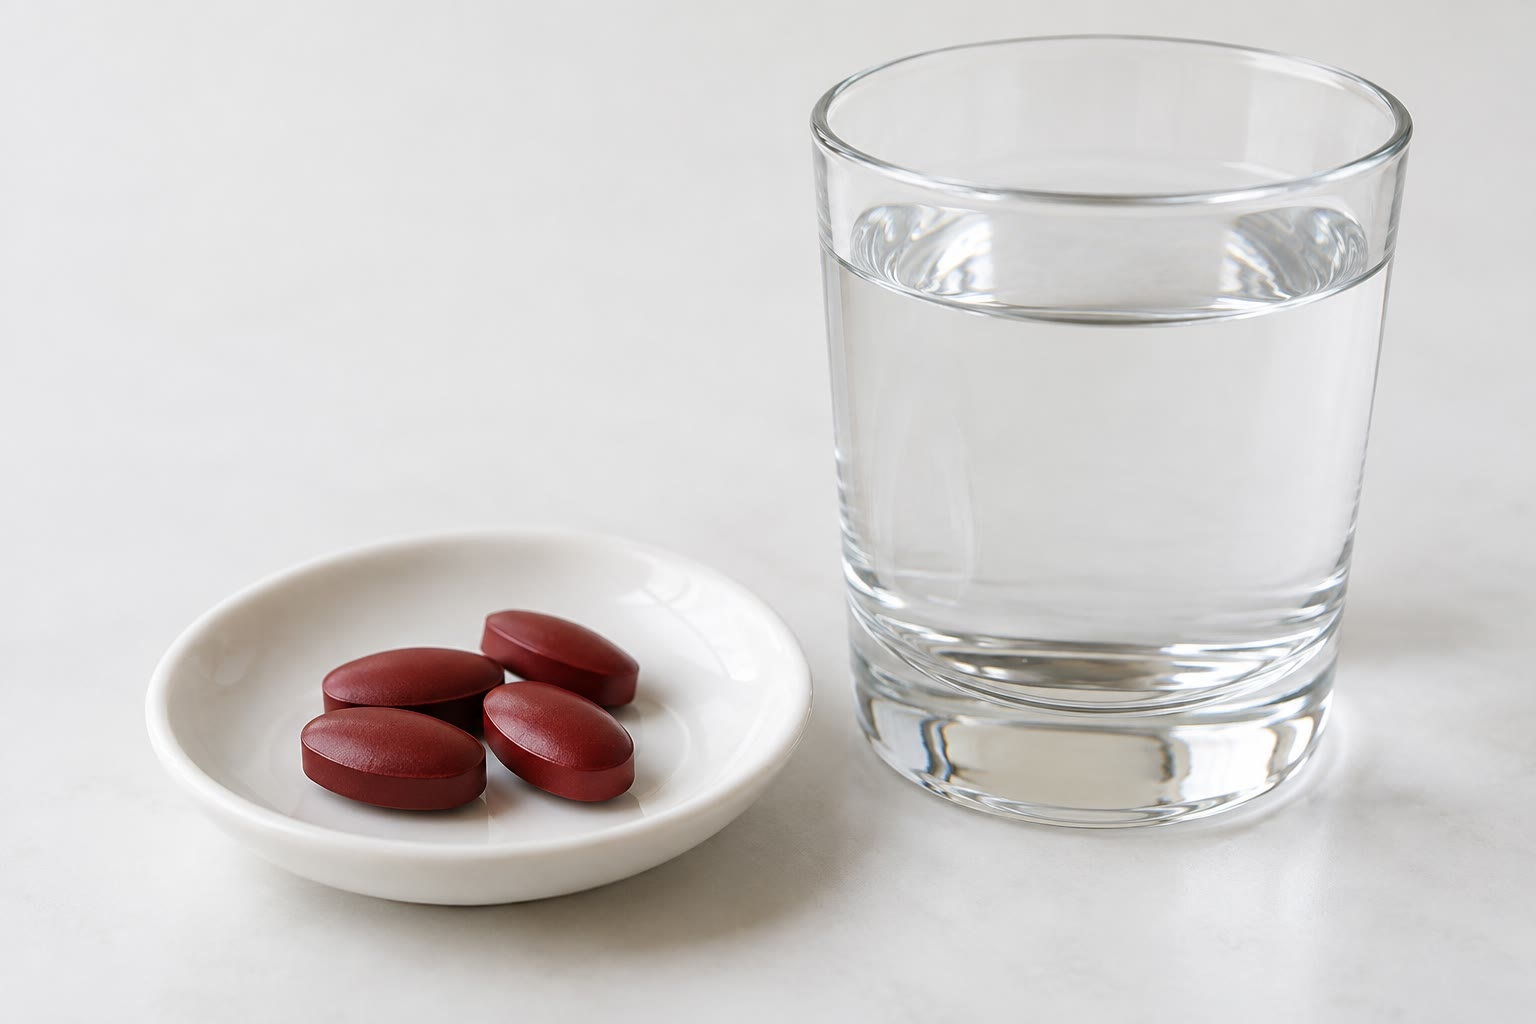
\includegraphics[width=0.45\linewidth]{images/book1/ai/g11-iron-tablets.jpg}

{\small أقراص مكمّل الحديد: كم من الحديد يحوي كل قرص حقًا؟}
\end{omfigure}

\section{المعايرة}

\begin{definition}[المعايرة، المحلول المعايِر، المحلول المراد معايرته]\label{def:g11:titration:titration}
\emph{المعايرة}\index{معايرة} تقيس كمية \omterm{def:g6:pure-substances-and-mixtures:species}{نوع كيميائي} \omterm{def:g6:solutions-and-solubility:solute}{مذاب}
بجعله يتفاعل مع \omterm{def:g6:pure-substances-and-mixtures:species}{نوع كيميائي} آخر تركيزه معروف
بدقة. \omterm{def:g2:mixing-and-dissolving:dissolve}{والمحلول} المعروف التركيز، الذي يُضاف من
السحاحة، هو \emph{المحلول المعايِر}\index{محلول معاير}؛ \omterm{def:g2:mixing-and-dissolving:dissolve}{والمحلول} الذي يحوي
النوع المراد قياسه، الموضوع في الدورق، هو \emph{المحلول المراد
معايرته}\index{محلول مراد معايرته}.
\end{definition}

\begin{proposition}[ما يجب أن يكون عليه تفاعل المعايرة]\label{prop:g11:titration:conditions}
يصلح التفاعل \omterm{def:g11:titration:titration}{للمعايرة} إذا كان تامًا (بحيث يُستهلك أحد
المتفاعلين كليًا)، وسريعًا (بحيث تتفاعل كل قطرة فورًا)،
ووحيدًا (فلا يتفاعل \omterm{def:g11:titration:titration}{المحلول المعايِر} مع أي شيء آخر في الدورق).
\end{proposition}

\begin{proof}
لو توقف التفاعل قبل اكتماله، أو تأخر عن القطرات،
أو استهلك المحلولَ المعايِر في غير موضعه، لما عاد الحجم المسكوب يقيس
كمية النوع المراد معايرته.
\end{proof}

\begin{omfigure}
\begin{tikzpicture}[font=\small, scale=0.62]
  \pic[transform shape] at (0,0) {stand={5.8}{1.8}};
  \pic[transform shape] at (1.8,0.68) {stirrer};
  \pic[transform shape] at (1.8,0.68) {erlenmeyer={0.25}{yellow!12}};
  \pic[transform shape] at (1.8,2.98) {burette={0.75}{violet!55}};
  \draw[omProp, thick, <-] (2.15,6.9) -- (4.2,7.4) node[right, text=black,
    align=left] {السحاحة: المحلول المعايِر\\ (برمنغنات البوتاسيوم)};
  \draw[omProp, thick, <-] (2.55,1.4) -- (4.2,1.9) node[right, text=black,
    align=left] {الدورق المخروطي: المحلول المراد\\ \foreignlanguage{arabic}{معايرته (الحديد \babelsublr{(II)}، حمض)}};
  \draw[omProp, thick, <-] (3.0,0.4) -- (4.2,0.3) node[right, text=black]
    {مخلاط مغناطيسي};
\end{tikzpicture}

{\small تجهيزة \omterm{def:g11:titration:titration}{معايرة}: السحاحة، المثبتة على حامل، تصبّ
\omterm{def:g11:titration:titration}{المحلول المعايِر} في \omterm{def:g11:titration:titration}{المحلول المراد معايرته}، الذي يُبقى مُحرَّكًا.}
\end{omfigure}

\section{التكافؤ}

\begin{definition}[التكافؤ، حجم التكافؤ]\label{def:g11:titration:equivalence}
\emph{التكافؤ}\index{تكافؤ} لحظة من \omterm{def:g11:titration:titration}{المعايرة} يكون فيها
\omterm{def:g11:titration:titration}{المحلول المعايِر} المضاف والنوع المراد معايرته بنسب
المعادلة: فيُستهلكان كلاهما. وحجم \omterm{def:g11:titration:titration}{المحلول المعايِر} المسكوب في تلك اللحظة
هو \emph{حجم التكافؤ}\index{حجم التكافؤ}، $V_E$.
\end{definition}

\begin{proposition}[العلاقة عند التكافؤ]\label{prop:g11:titration:relation}
لتفاعل \omterm{def:g11:titration:titration}{معايرة} $a\,\ce{A} + b\,\ce{B} \longrightarrow \text{نواتج}$، يُعايَر فيه A (كميته
$n_A$) \omterm{def:g2:mixing-and-dissolving:dissolve}{بمحلول} معايِر B تركيزه $c_B$، يكون عند \omterm{def:g11:titration:equivalence}{التكافؤ}
\[
  \frac{n_A}{a} = \frac{c_B\, V_E}{b} .
\]
\end{proposition}

\begin{proof}
عند \omterm{def:g11:titration:equivalence}{التكافؤ} يكون \omterm{def:g6:pure-substances-and-mixtures:mixture}{الخليط} بالنسب الستوكيومترية
(\cref{ch:g10:reaction-progress-table}): فالنوعان A وB، وكميتاهما الابتدائيتان $n_A$
و$c_B V_E$، ينفدان معًا، إذن $n_A / a = c_B V_E / b$.
\end{proof}

\begin{omfigure}
\begin{tikzpicture}
\begin{axis}[width=0.72\linewidth, height=5.6cm, xmin=0, xmax=20,
    ymin=0, ymax=16, xlabel={\foreignlanguage{arabic}{حجم المحلول المعايِر المضاف \babelsublr{(\si{mL})}}},
    ylabel={\foreignlanguage{arabic}{الكمية \babelsublr{($\num{e-4}$ \si{mol})}}}, axis lines*=left, ymajorgrids,
    grid style={gray!20}, tick label style={font=\small},
    label style={font=\small}, legend style={font=\small, at={(0.98,0.97)},
    anchor=north east, draw=none}, legend cell align=left]
  \addplot[very thick, orange!70!black, domain=0:14.3] {14.3 - x};
  \addplot[very thick, violet, domain=14.3:20] {0.2*(x - 14.3)};
  \addplot[very thick, violet, domain=0:14.3, forget plot] {0};
  \legend{{\foreignlanguage{arabic}{\ce{Fe^{2+}} المتبقي في الدورق}}, {\foreignlanguage{arabic}{\ce{MnO4^-} بفائض}}}
  \addplot[dashed, black!60] coordinates {(14.3,0) (14.3,7)};
  \node[font=\small, anchor=west] at (axis cs:14.5,6.5) {$V_E = \qty{14.3}{mL}$};
\end{axis}
\end{tikzpicture}

{\small \omterm{def:g11:titration:titration}{معايرة} الحديد (II) بالبرمنغنات ذات التركيز \qty{0.0200}{mol/L}: تنفد
\omterm{def:g9:ions:ion}{أيونات} الحديد (II) تمامًا عند \omterm{def:g11:titration:equivalence}{حجم التكافؤ}؛ وبعده لا تعود
\omterm{def:g9:ions:ion}{أيونات} البرمنغنات تُستهلك فتتراكم.}
\end{omfigure}

\section{تحديد التكافؤ بتغير اللون}


\begin{proposition}[رؤية التكافؤ]\label{prop:g11:titration:colour}
حين يكون أحد أنواع \omterm{def:g11:titration:titration}{المعايرة} ملوّنًا، يُرى \omterm{def:g11:titration:equivalence}{التكافؤ}
تغيرًا في لون الدورق: فإما أن يظهر لون \omterm{def:g11:titration:titration}{المحلول المعايِر}
ويثبت ما إن يصير بفائض، وإما أن يختفي لون النوع
المراد معايرته حين ينفد.
\end{proposition}

\begin{proof}
قبل \omterm{def:g11:titration:equivalence}{التكافؤ}، يُستهلك فورًا كل \omterm{def:g9:ions:ion}{أيون} من \omterm{def:g11:titration:titration}{المحلول المعايِر} يسقط في
الدورق؛ وبعد \omterm{def:g11:titration:equivalence}{التكافؤ} يبقى. فالنوع الملوّن
لا يوجد في الدورق إلا في جهة واحدة من \omterm{def:g11:titration:equivalence}{التكافؤ}.
\end{proof}

\begin{example}[البرمنغنات كاشفُ نفسها]\label{ex:g11:titration:permanganate}
\omterm{def:g9:ions:ion}{أيون} البرمنغنات \ce{MnO4^-} بنفسجي داكن، \omterm{def:g9:ions:ion}{وأيونات} المنغنيز
\ce{Mn^{2+}} التي يعطيها تكاد تكون عديمة اللون؛ ولا تعطي \omterm{def:g9:ions:ion}{أيونات} الحديد
\omterm{def:g2:mixing-and-dissolving:dissolve}{المحلول} إلا مسحة صفراء باهتة. فقبل \omterm{def:g11:titration:equivalence}{التكافؤ}، تفقد كل قطرة بنفسجية
لونها حين تسقط؛ وأول قطرة لا تفقده تُعلن
\omterm{def:g11:titration:equivalence}{التكافؤ}: فيصير الدورق ورديًا باهتًا ويبقى كذلك.
\end{example}

\begin{omfigure}
\begin{tikzpicture}[font=\small]
  \pic at (0,0) {erlenmeyer={0.3}{yellow!14}};
  \pic at (3.2,0) {erlenmeyer={0.3}{magenta!10}};
  \pic at (6.4,0) {erlenmeyer={0.3}{violet!45}};
  \node[align=center, anchor=north] at (0,-0.15) {قبل التكافؤ:\\
    أصفر باهت، وكل قطرة\\ تفقد لونها};
  \node[align=center, anchor=north] at (3.2,-0.15) {عند التكافؤ:\\
    وردي خفيف\\ يثبت};
  \node[align=center, anchor=north] at (6.4,-0.15) {بعد التكافؤ:\\
    بنفسجي، والبرمنغنات\\ بفائض};
\end{tikzpicture}

{\small دورق \omterm{def:g11:titration:titration}{معايرة} الحديد (II) بالبرمنغنات، قبل \omterm{def:g11:titration:equivalence}{التكافؤ} وعنده
وبعده. ويُقرأ \omterm{def:g11:titration:equivalence}{حجم التكافؤ} عند أول لون وردي
ثابت.}
\end{omfigure}

\begin{example}[فيتامين C وثنائي اليود]\label{ex:g11:titration:vitamin-c}
% ledger: aw:C, aw:H, aw:O
فيتامين C، أي حمض الأسكوربيك \ce{C6H8O6} ($M = \qty{176.0}{g/mol}$)،
\omterm{def:g11:redox:oxidant}{مختزل}؛ وثنائي اليود \ce{I2} يؤكسده:
\[
  \ce{C6H8O6 + I2 -> C6H6O6 + 2H+ + 2I-} .
\]
يُعايَر \qty{10.0}{mL} من عصير البرتقال، مع قليل من النشا، \omterm{def:g2:mixing-and-dissolving:dissolve}{بمحلول}
ثنائي اليود تركيزه \qty{5.00e-3}{mol/L}. قبل \omterm{def:g11:titration:equivalence}{التكافؤ} يُستهلك ثنائي
اليود؛ وأول قطرة بفائض تُلوّن النشا بالأزرق الداكن. فإذا كان
$V_E = \qty{5.70}{mL}$، فقد احتوى العصير
$n = \num{5.00e-3} \times \num{5.70e-3} = \qty{2.85e-5}{mol}$ من فيتامين
C، أي \qty{5.0}{mg} في \qty{10.0}{mL}: \qty{0.50}{g/L}.
\end{example}

\section{حساب تركيز مجهول}

\begin{method}[حساب تركيز من معايرة]\label{met:g11:titration:computing}
\begin{enumerate}
  \item اكتب \omterm{def:g8:balanced-equations:equation}{المعادلة الموزونة} لتفاعل \omterm{def:g11:titration:titration}{المعايرة} واقرأ
        المعاملين $a$ (النوع المراد معايرته) و$b$ (\omterm{def:g11:titration:titration}{المحلول المعايِر}).
  \item اقرأ $V_E$ على السحاحة، واحسب كمية \omterm{def:g11:titration:titration}{المحلول المعايِر}
        المسكوبة، $n_B = c_B V_E$.
  \item عند \omterm{def:g11:titration:equivalence}{التكافؤ}، $n_A = \dfrac{a}{b}\, c_B V_E$.
  \item اقسم على الحجم المعايَر: $c_A = n_A / V_A$. وإذا كانت العيّنة
        قد خُففت قبل \omterm{def:g11:titration:titration}{المعايرة}، فاضرب في \omterm{def:g10:concentration-and-dilution:dilution}{معامل التخفيف}.
\end{enumerate}
\end{method}

\begin{example}[محلول من الحديد (II)]\label{ex:g11:titration:iron}
يتطلب \qty{20.0}{mL} من \omterm{def:g2:mixing-and-dissolving:dissolve}{محلول} محمَّض من الحديد (II)
$V_E = \qty{12.6}{mL}$ من البرمنغنات ذات التركيز \qty{0.0200}{mol/L}. وهنا
$a = 5$ (\ce{Fe^{2+}}) و$b = 1$ (\ce{MnO4^-}):
$n(\ce{MnO4^-}) = 0.0200 \times 0.0126 = \qty{2.52e-4}{mol}$، إذن
$n(\ce{Fe^{2+}}) = 5 \times \num{2.52e-4} = \qty{1.26e-3}{mol}$،
و$c(\ce{Fe^{2+}}) = \num{1.26e-3} / 0.0200 = \qty{0.0630}{mol/L}$.
\end{example}

\section{المعايرة بوصفها قياسًا}

\begin{inthelab}[قراءة السحاحة]
تُشطف السحاحة \omterm{def:g11:titration:titration}{بالمحلول المعايِر}، وتُملأ، وتُخلّص فوهتها من فقاعات
\omterm{def:g4:air-a-mixture-of-gases:air}{الهواء}. ويُقرأ المستوى عند أسفل الهلالة، والعين
على الارتفاع نفسه، قبل \omterm{def:g11:titration:titration}{المعايرة} وبعدها: والحجم المسكوب هو
الفرق. والتدريجات كل \qty{0.1}{mL}، ويمكن تقدير القراءة
إلى \qty{0.05}{mL}. وقرب \omterm{def:g11:titration:equivalence}{التكافؤ} يُضاف \omterm{def:g11:titration:titration}{المحلول المعايِر} قطرةً
قطرةً، مع رجّ الدورق أو تحريكه.
\end{inthelab}

\begin{omfigure}
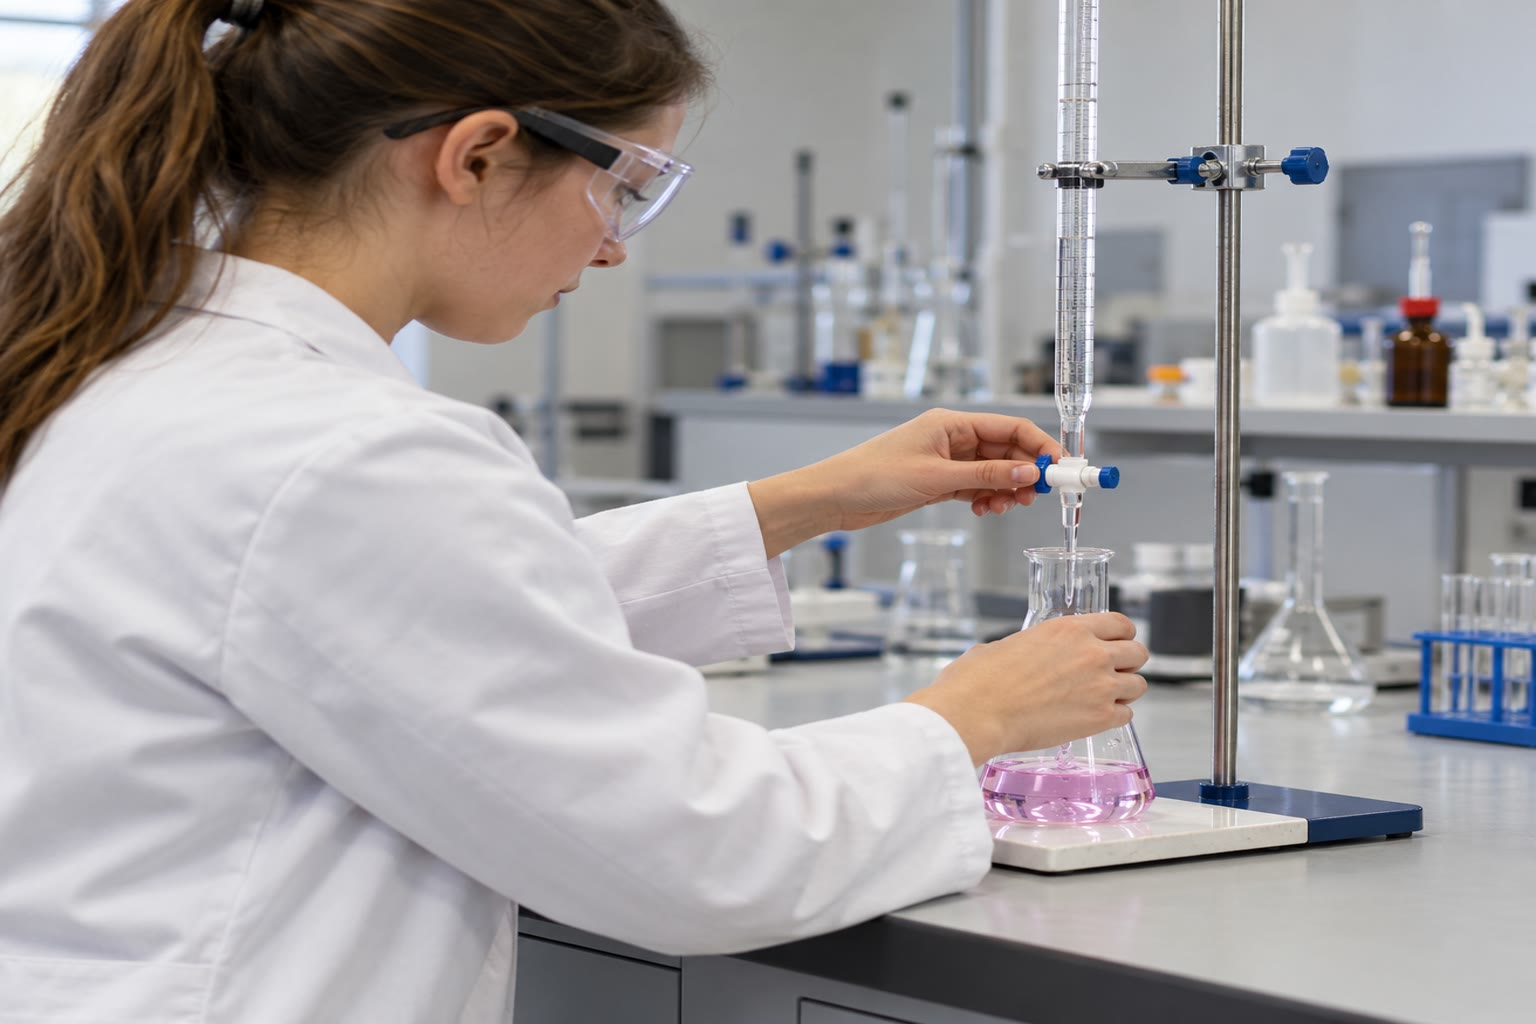
\includegraphics[width=0.48\linewidth]{images/book1/ai/g11-titration-bench.jpg}

{\small \omterm{def:g11:titration:titration}{معايرة} جارية: سحاحة وحامل ودورق مخروطي على
بلاطة بيضاء.}
\end{omfigure}

\begin{remark}[ما مدى دقة المعايرة؟]\label{rem:g11:titration:precision}
قد تخطئ كل قراءة للسحاحة بنحو \qty{0.05}{mL}، والحجم
المسكوب فرق بين قراءتين: فقد يخطئ بما يصل إلى \qty{0.1}{mL}.
ففي حالة $V_E = \qty{14.3}{mL}$ يكون ذلك $0.1 / 14.3 \approx
\qty{0.7}{\percent}$. وكلما كبر $V_E$ صغر هذا الخطأ النسبي،
ولذلك تُختار تراكيز المحاليل المعايِرة بحيث تعطي أحجام \omterm{def:g11:titration:equivalence}{تكافؤ}
من 10 إلى \qty{20}{mL} مع سحاحة سعتها \qty{25}{mL}. وتُكرَّر
\omterm{def:g11:titration:titration}{المعايرة} حتى تتفق نتيجتان في حدود نحو
\qty{0.1}{mL}. ويعالج مجلد السنة الأولى عدم اليقين في القياس معالجة
أدق.
\end{remark}

\begin{safety}{\ghs[0.7cm]{GHS03}\ghs[0.7cm]{GHS05}\ghs[0.7cm]{GHS07}\ghs[0.7cm]{GHS08}\ghs[0.7cm]{GHS09}}
% ledger: ghs:KMnO4, ghs:I2
برمنغنات البوتاسيوم الصلبة \omterm{def:g11:redox:oxidant}{مؤكسد} قد يغذي حريقًا،
وهي أكّالة وضارة؛ ومحاليلها المخففة تصبغ الجلد والملابس
بالبني. ومحاليل ثنائي اليود ضارة. نظارتان واقيتان وقفازان؛ وتُجمع النفايات،
ولا تُسكب أبدًا في المغسلة.
\end{safety}

\section{تمارين}


\begin{exercise}[$\star$]\label{exo:g11:titration:1}
ما \omterm{def:g11:titration:titration}{المحلول المعايِر} في \omterm{def:g11:titration:titration}{المعايرة}؟ وما \omterm{def:g11:titration:titration}{المحلول المراد معايرته}؟ وماذا يحدث
عند \omterm{def:g11:titration:equivalence}{التكافؤ}؟
\end{exercise}

\begin{exercise}[$\star$]\label{exo:g11:titration:2}
ما كمية \omterm{def:g9:ions:ion}{أيونات} البرمنغنات التي يحويها \qty{12.5}{mL} من
\omterm{def:g2:mixing-and-dissolving:dissolve}{محلول} تركيزه \qty{0.0200}{mol/L}؟
\end{exercise}

\begin{exercise}[$\star$]\label{exo:g11:titration:3}
اقرأ \omterm{def:g11:titration:equivalence}{حجم التكافؤ} على شكل الكميات بدلالة الحجم المسكوب.
وما كمية الحديد (II) التي كانت في الدورق في
البداية؟
\end{exercise}

\begin{exercise}[$\star$]\label{exo:g11:titration:4}
لماذا لا حاجة إلى كاشف ملوّن في \omterm{def:g11:titration:titration}{المعايرة} بالبرمنغنات؟
\end{exercise}

\begin{exercise}[$\star$]\label{exo:g11:titration:5}
عند \omterm{def:g11:titration:equivalence}{التكافؤ} في \omterm{def:g11:titration:titration}{معايرة} الحديد (II) بالبرمنغنات، ما
النسبة بين كمية الحديد (II) وكمية البرمنغنات
المسكوبة؟ ولماذا؟
\end{exercise}

\begin{exercise}[$\star\star$]\label{exo:g11:titration:6}
يتطلب \qty{10.0}{mL} من \omterm{def:g2:mixing-and-dissolving:dissolve}{محلول} محمَّض من الحديد (II) \qty{8.40}{mL} من
البرمنغنات ذات التركيز \qty{0.0200}{mol/L}. احسب \omterm{def:g10:concentration-and-dilution:molar-concentration}{التركيز المولي}
للحديد (II)، ثم تركيزه الكتلي.
\end{exercise}

\begin{exercise}[$\star\star$]\label{exo:g11:titration:7}
يُذاب قرص من فيتامين C لتحضير \qty{100.0}{mL} من \omterm{def:g2:mixing-and-dissolving:dissolve}{المحلول}.
ويتطلب \qty{10.0}{mL} منه، مع النشا، \qty{11.4}{mL} من ثنائي اليود تركيزه
\qty{0.0100}{mol/L}. ما كتلة فيتامين C التي يحويها القرص؟
\end{exercise}

\begin{exercise}[$\star\star$]\label{exo:g11:titration:8}
\omterm{def:g10:reaction-progress-table:limiting}{تفاعل تام} لكنه يستغرق عدة دقائق. لماذا لا يمكن استعماله
كما هو في \omterm{def:g11:titration:titration}{معايرة} تعتمد على تغير اللون؟
\end{exercise}

\begin{exercise}[$\star\star$]\label{exo:g11:titration:9}
انظر إلى الدوارق الثلاثة. توقفت طالبة عند دورق بنفسجي كالدورق
الثالث. أحجم \omterm{def:g11:titration:equivalence}{التكافؤ} الذي وجدته أكبر مما ينبغي أم أصغر؟ وماذا كان
عليها أن تفعل قرب \omterm{def:g11:titration:equivalence}{التكافؤ}؟
\end{exercise}

\begin{exercise}[$\star\star$]\label{exo:g11:titration:10}
يُخفَّف أولًا \omterm{def:g2:mixing-and-dissolving:dissolve}{محلول} مركّز من الحديد (II) عشر مرات. ثم يتطلب
\qty{10.0}{mL} من \omterm{def:g2:mixing-and-dissolving:dissolve}{المحلول} المخفف \qty{13.0}{mL} من
البرمنغنات ذات التركيز \qty{0.0200}{mol/L}. جد تركيز
\omterm{def:g2:mixing-and-dissolving:dissolve}{المحلول} المركّز.
\end{exercise}

\begin{exercise}[$\star\star$]\label{exo:g11:titration:11}
% ledger: aw:Fe
تركيز \omterm{def:g2:mixing-and-dissolving:dissolve}{محلول} الحديد (II) في المثال \omterm{def:g2:mixing-and-dissolving:dissolve}{المحلول} في الفصل
$c = \qty{0.0630}{mol/L}$. ما كتلة الحديد التي يحويها \qty{1.00}{L}
منه؟
\end{exercise}

\begin{exercise}[$\star\star\star$]\label{exo:g11:titration:12}
أعطت \omterm{def:g11:titration:titration}{معايرة} $V_E = \qty{7.2}{mL}$. قدّر الخطأ النسبي \omterm{def:g7:chemical-reactions:reactant}{الناتج}
عن قراءات السحاحة، وقارنه بحالة $V_E = \qty{14.3}{mL}$. واقترح
طريقتين للحصول على حجم \omterm{def:g11:titration:equivalence}{تكافؤ} أكبر.
\end{exercise}

\begin{exercise}[$\star\star\star$]\label{exo:g11:titration:13}
يُعايَر بيروكسيد الهيدروجين بالبرمنغنات في وسط حمضي:
\[
  \ce{2MnO4^- + 5H2O2 + 6H+ -> 2Mn^{2+} + 5O2 + 8H2O} .
\]
يُخفَّف مطهِّر عشر مرات؛ ويتطلب \qty{10.0}{mL} من \omterm{def:g2:mixing-and-dissolving:dissolve}{المحلول}
المخفف \qty{17.6}{mL} من البرمنغنات ذات التركيز \qty{0.0200}{mol/L}.
جد \omterm{def:g10:concentration-and-dilution:molar-concentration}{التركيز المولي} لبيروكسيد الهيدروجين في المطهِّر،
ثم تركيزه الكتلي (\ce{H2O2}: \qty{34.0}{g/mol}).
\end{exercise}

\begin{exercise}[$\star\star\star$]\label{exo:g11:titration:14}
ينبغي أن يحوي قرص الحديد نحو \qty{1.4e-3}{mol} من الحديد (II). أي
تركيز للبرمنغنات يعطي حجم \omterm{def:g11:titration:equivalence}{تكافؤ} قريبًا من
\qty{15}{mL} مع سحاحة سعتها \qty{25}{mL}؟ وما الخلل الذي يقع مع
\omterm{def:g2:mixing-and-dissolving:dissolve}{محلول} أشد تركيزًا بعشر مرات؟
\end{exercise}

\begin{exercise}[$\star\star\star$]\label{exo:g11:titration:15}
تُظهر معادلة \omterm{def:g11:titration:titration}{المعايرة} \ce{8H+} لكل \ce{MnO4^-}. فلحجم
\omterm{def:g11:titration:equivalence}{تكافؤ} قدره \qty{14.3}{mL} بتركيز \qty{0.0200}{mol/L}، ما كمية
\omterm{def:g9:ions:ion}{أيونات} الهيدروجين المستهلكة؟ وهل تكفي \qty{10}{mL} من حمض يحوي
\qty{1.0}{mol/L} من \omterm{def:g9:ions:ion}{أيونات} الهيدروجين؟ ولماذا يجب تحميض
الدورق؟
\end{exercise}

\section{مسألة: أصادقٌ قرص الحديد؟}

\begin{problem}[{مسألة نهاية الأسبوع --- مكمّل حديد يَعِد بأن في القرص 80 mg
من الحديد: أتؤيد المعايرة ذلك؟}]
\label{pb:g11:titration:1}
% ledger: aw:Fe, aw:S, aw:O, const:NA
تَعِد علبة مكمّل الحديد بأن في كل قرص \qty{80}{mg} من الحديد، على هيئة
الحديد (II). يُسحق قرص ويُذاب في نحو \qty{50}{mL} من
حمض الكبريتيك المخفف، ثم يُعايَر ببرمنغنات البوتاسيوم ذات التركيز
\qty{0.0200}{mol/L}. فيثبت اللون الوردي الخفيف عند $V_E = \qty{14.3}{mL}$.

\medskip
\noindent\textbf{الجزء الأول --- التفاعل.}
\begin{enumerate}
  \item سمِّ مزدوجتي \omterm{def:g11:redox:oxidation}{الأكسدة} \omterm{def:g11:redox:oxidation}{والاختزال} المعنيتين. أي النوعين
        \omterm{def:g11:redox:oxidant}{المؤكسد}، وأيهما \omterm{def:g11:redox:oxidant}{المختزل}؟
  \item اكتب نصفي المعادلتين.
  \item اجمعهما في معادلة \omterm{def:g11:titration:titration}{المعايرة}، وتحقق من أنها
        موزونة في الشحنة.
  \item لماذا يُذاب القرص في حمض؟
  \item بيّن أن التفاعل يحقق شروط \omterm{def:g11:titration:titration}{المعايرة}،
        واشرح كيف يُرى \omterm{def:g11:titration:equivalence}{التكافؤ}.
\end{enumerate}

\medskip
\noindent\textbf{الجزء الثاني --- \omterm{def:g11:titration:titration}{المعايرة}.}
\begin{enumerate}[resume]
  \item في أي أداة زجاجية يوجد \omterm{def:g2:mixing-and-dissolving:dissolve}{محلول} البرمنغنات؟ وكيف
        يُقرأ حجمه؟
  \item ما لون الدورق قبل \omterm{def:g11:titration:equivalence}{التكافؤ}، ولماذا تفقد كل
        قطرة لونها؟
  \item احسب كمية البرمنغنات المسكوبة عند \omterm{def:g11:titration:equivalence}{التكافؤ}.
\end{enumerate}

\medskip
\noindent\textbf{الجزء الثالث --- الحديد.}
\begin{enumerate}[resume]
  \item استنتج كمية الحديد (II) في القرص.
  \item احسب كتلته بالمليغرام.
  \item قارن باللصاقة: ما الفرق النسبي؟
  \item قد يخطئ الحجم المسكوب بمقدار \qty{0.1}{mL}. فبكم
        مليغرامًا قد تخطئ كتلة الحديد؟ وهل تأكدت صحة اللصاقة؟
\end{enumerate}

\medskip
\noindent\textbf{الجزء الرابع --- عدة أقراص.}
\begin{enumerate}[resume]
  \item يعطي قرصان آخران $V_E = \qty{14.1}{mL}$
        و\qty{14.4}{mL}. احسب كتلتي الحديد فيهما.
  \item احسب متوسط الأقراص الثلاثة.
  \item تختلف النتائج الثلاث بأكثر من خطأ السحاحة. فماذا
        يدل ذلك على الأقراص؟
  \item أكانت البرمنغنات ذات التركيز \qty{0.100}{mol/L} اختيارًا
        أفضل؟ اشرح.
  \item كثير من المكملات تحوي أيضًا فيتامين C، وهو \omterm{def:g11:redox:oxidant}{مختزل}. فماذا
        يفعل \omterm{def:g11:titration:titration}{بالمعايرة}، وبكتلة الحديد المحسوبة؟
  \item الحديد موجود على هيئة كبريتات الحديد (II)، \ce{FeSO4}. ما الكتلة
        التي يحويها القرص الواحد منها؟
  \item كم أيونًا من الحديد (II) يمثل ذلك؟
  \item اذكر الجواب النهائي: ما كتلة الحديد التي يحويها القرص
        الواحد؟
\end{enumerate}
\end{problem}
